\documentclass[conference]{IEEEtran}
\usepackage{amsmath,amssymb,amsfonts}
\usepackage{algorithmic}
\usepackage{graphicx}
\usepackage{textcomp}
\usepackage{xcolor}

\usepackage[numbers]{natbib}
\usepackage{hyperref}
\usepackage{url}
\usepackage{dblfloatfix}
\usepackage{booktabs}
\usepackage{makecell}
\usepackage{footnote}
\usepackage{pgf-pie}
\def\BibTeX{{\rm B\kern-.05em{\sc i\kern-.025em b}\kern-.08em
		T\kern-.1667em\lower.7ex\hbox{E}\kern-.125emX}}
\bibliographystyle{ieeetr}


\begin{document}
	\title{A Survey on Hardware Accelerators for Neural Networks}
	\author{
		\IEEEauthorblockN{Pierre Brosemer}
		\IEEEauthorblockA{uitxj@student.kit.edu}
	}
	
	\maketitle
	
	\begin{abstract}
		Neural networks are a widely used method in the field of Artificial Intelligence. With the ability to beat the best human players at the complicated game of GO \cite{chouard2016go} neural networks are becoming a high performing tool to solve a variety of problems. Their tradeoff: they require vast amounts of computational power, creating the need for hardware accelerators. This work provides a state-of-the-art survey on the main types of hardware presenting recent products for each of the categories and concludes by comparing each of them. First, the basics of neural networks are covered in order to understand the reasoning behind the hardware design choices, followed by the technical implementations.
		\\
	\end{abstract}
	
	\section{Introduction}
	Artificial neural networks (more often neural networks) are one of the most promising technologies in the current era of computer science. Neural networks can be deployed in an enormous variety of categories and have shown major improvements in these categories, most prominently in speech and image recognition \cite{speech_recognition1} that exceeded prior methods. The field of Artificial Intelligence covers a wide variety of concepts. This paper will mainly cover the subcategory of Deep Learning, more specifically neural networks, which falls under the category of Machine Learning. 
	\\
	Neural networks are at its core a very broad simplification of the biological brain consisting of many interconnected neurons, called nodes in neural networks. The nodes in a neural network are   arranged in different layers. Each node passes on a weighted function to a node in the next layer. If this value is above a certain threshold the node will be activated. The activation function then determines the output of this node, depending on the inputs. There are many different activation functions that are chosen by the type of neural network. By changing the weights of each node a learning process similar to that of their biological counterpart is simulated \cite{nn_basics}.
	\begin{figure}[h]
		\caption{A typical representation of a neural network. The input layer gives the raw input to the next layer, where nodes process the input and give their output to the next layer. The last layer results in an output (the result)}
		\centering
		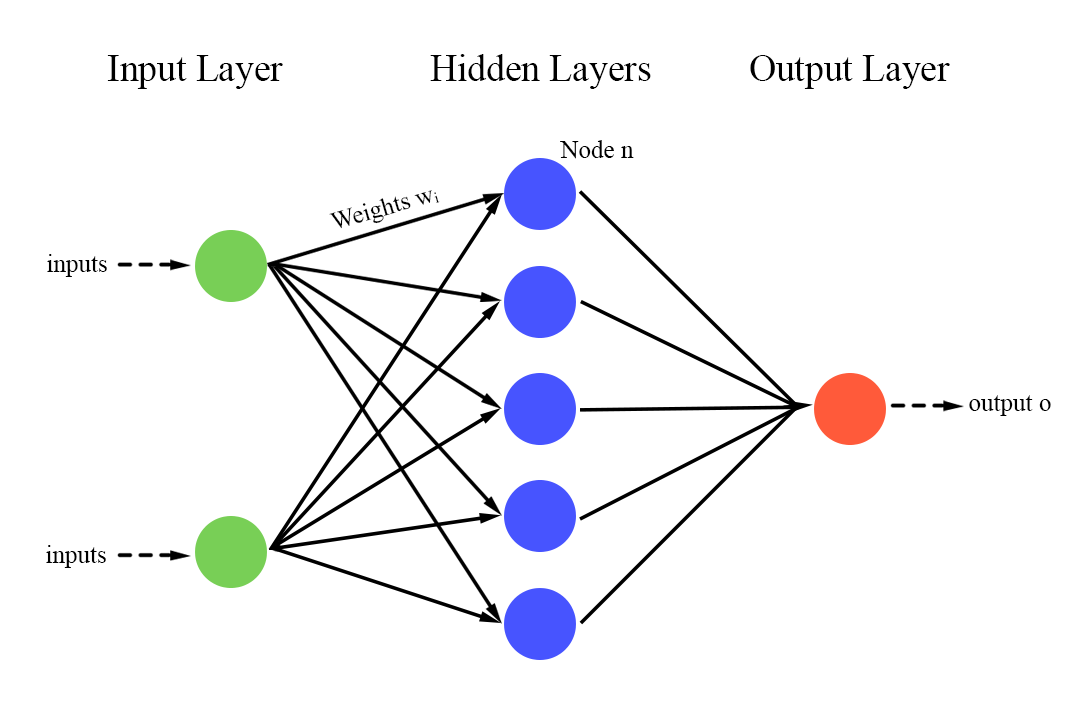
\includegraphics[width=\linewidth]{pictures/neuralnetwork.png}
	\end{figure}
	\\
	The development of a neural network consists of two different stages. Firstly, a training phase where the neural network receives an input and compares the resulting output (prediction) with that of a real-world dataset. The error can then be incorporated into the network by changing the different weights. The algorithm that has the task of changing the weights is called the backpropagation algorithm. Secondly, an inference phase, where the network receives an input and makes a prediction. The neural network has a larger computational demand in the training phase as more data is processed, as well as the weights needing calibration.
	\\
	\\
	With some neural networks having over 150 layers \cite{densely_network} up to billions of multiplications can take place in a single neural network and one propagation. The vast amount of computational power needed for training and using neural network lead to the need for specialized hardware, which contributed much to the success seen in modern day implementations. The research on hardware is still ongoing and is one of the most important topics in achieving better and faster results for neural networks. As a result of the timeliness of the topic this survey will only cover a status quo of the current hardware.
	\\
	
	\section{Different Types of Hardware}
	Most of computations needed for inference and training include matrix-vector products, caused by the input data being run through the network.
	Furthermore, the dimension of the input data plays a key role in the amount of computation needed. Assuming a single image has 1000 pixels resulting in 1000 different data points that the neural network has to compute. To efficiently compute the vast amount of data, fast memory accesses or in- place computations of the values are needed. Since these calculations need to be done for the number of nodes, good parallelization is needed to run neural networks efficiently.
	\\
	Hardware accelerators for neural networks can be divided into four main classes: CPUs, GPUs, FPGAs and ASICs. The focus can be placed on the latter three, since CPUs mostly fall short in terms of computational power for neural networks. 
	CPUs are needed for a wide variety of tasks requiring a flexible system to execute instructions. As a result a CPU is good at executing serial instructions in parallel, resulting in a good general parallelization.
	Both of the points mentioned above, that are needed for the specialized hardware for neural networks, are not met for CPUs. They are limited by their small amount of cores hindering the ability to parallelize the same instruction. Moreover, a CPU usually works by fetching an instruction and executing it making the training and inference phase slow \cite{capra2020updated}. While working on neural networks CPUs are accompanied by underutilization, achieving factors of less than 1/10 of that of other alternatives \cite{nurvitadhi2016accelerating}. Nonetheless, Intel is working on accelerating CPUs producing libraries for their Intel Xeon Processor \cite{intelnn}.
	\\
	Another point to consider is the different requirements needed for both the training and inference phase. During the inference phase certain approximations can be made to achieve faster results, which cannot be made for the training phase. This derives in some hardware only being designed for the inference phase \cite{jouppi2017datacenter}. 
	\\
	Additionally the hardware can be divided into spatial architectures and temporal architectures \cite{sze2017efficient}. 
	CPUs and GPUs mostly are built on the premise of temporal architecture. Temporal architectures have on central control system for many different Arithmic Logic Units (ALUs), as seen in Figure \ref{fig:archcomparison}. One ALU only communicates with the memory hierarchy, not with other units. In order to parallelize the workload execution models like SIMD (Single instruction, multiple data) or SIMT (Single instruction, multiple threads) are used. SIMD executes one operation on multiple Data at the same time. SIMT uses SIMD together with multithreading and is implemented in GPUs. 
	ASICs and FPGAs are built on spatial architectures. The different ALUs are connected together to and form a network, that can pass data from one ALU to the next. In spatial architectures ALUs can also have their own control and logic memory. A processing element or processing engine (PE) is an ALU with it's own local memory.
	
	\begin{figure}[b]
		\centering
		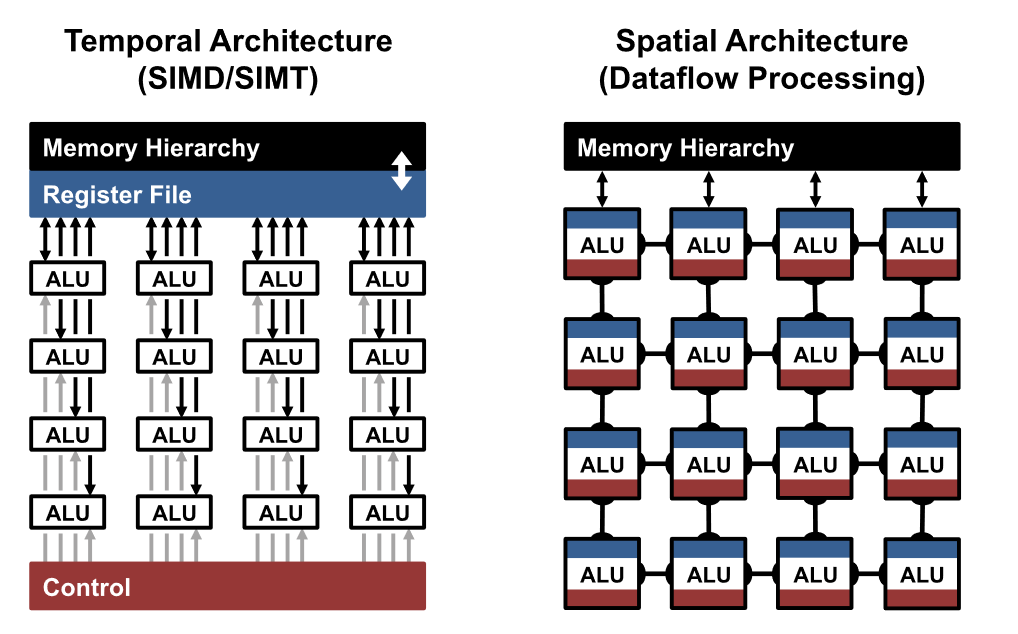
\includegraphics[width=\linewidth]{pictures/diff_architectures.png}
		\label{fig:archcomparison}
		\caption{A comparison between the different architecture types. The ALUs from the temporal architecture can only fetch data from the memory hierarchy \cite{sze2017efficient}.}
	\end{figure}
	
	\section{Graphics Processing Unit}
	The Graphics Processing Unit (GPU) is a piece of specialized hardware originally designed for the rendering of images in a computer. The rendering process requires vast amounts of floating point operations resulting in the GPU having hundreds of cores with many individual caches to store the computation. To add on the GPU has more units dedicated to floating-point operations. This makes the GPU an excellent tool for working with neural networks since the specifications align with those for rendering graphics. With over thousand cores the GPU can parallelize the matrix multiplications needed for training and achieve fast training times. 
	\begin{figure}[h]
		\caption{Different layouts comparing CPU and GPU: The GPU has more cores with more individual caches \cite{intelpic_comparison}}
		\centering
		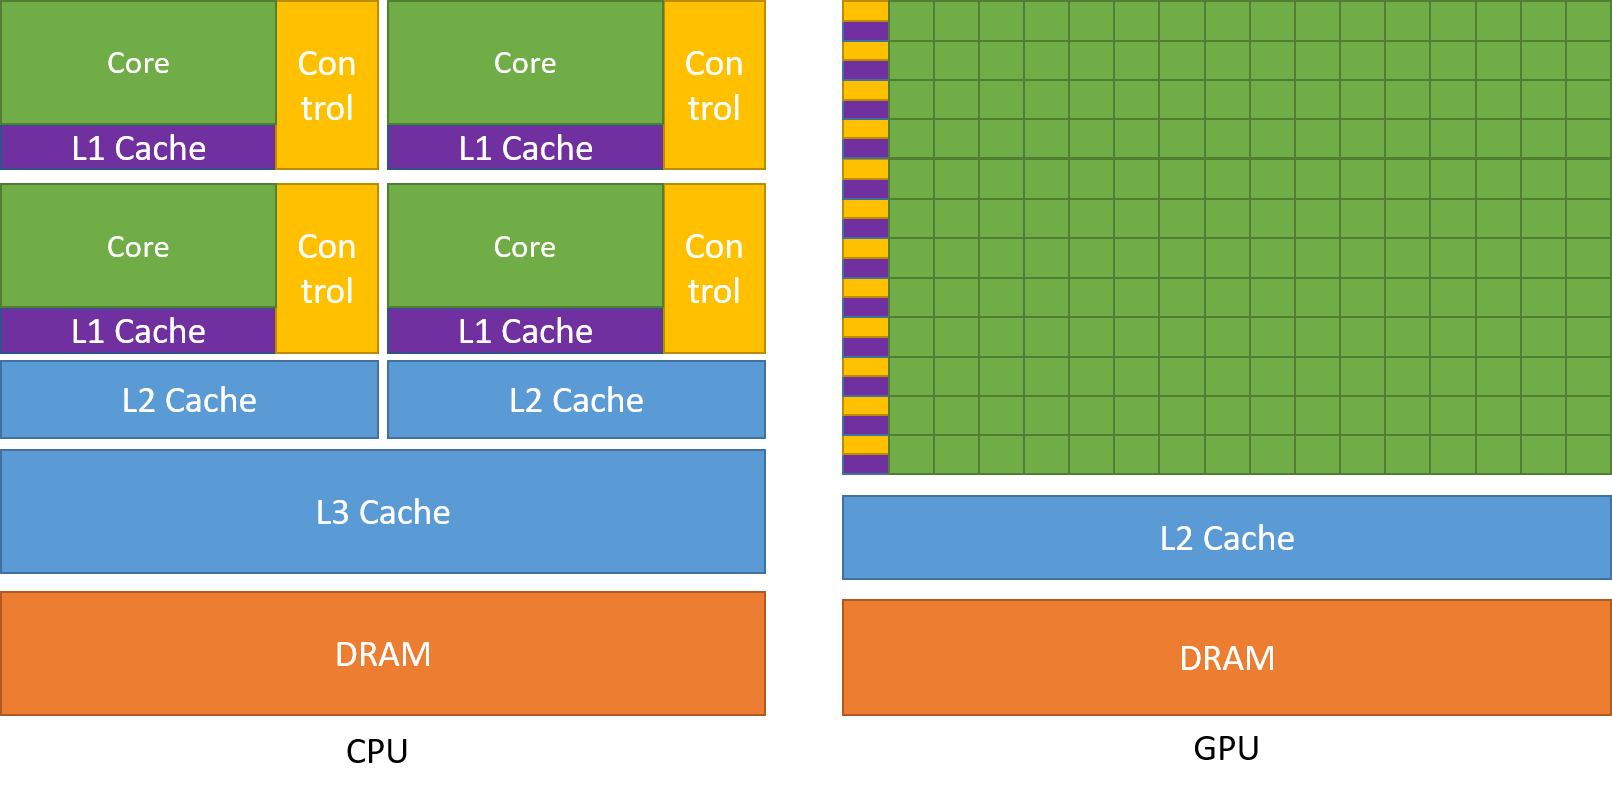
\includegraphics[width=\linewidth]{pictures/intel_comparison.png}
	\end{figure}
	\\
	Through this structure high memory throughput and good execution of parallel instructions is given. Nvidia, one of the leaders in manufacturing, is implementing its specialized Deep Learning Units with normal cores plus additional Tensor cores \cite{nvidiav100}. Tensor cores essentially multiply 2 FP-16 matrix (floating point 16 bit) and being able to add a third matrix all in a single operation, performing 64 operations per clock \cite{tensorcores}. Their newest product the Nvidia A100 uses the third generation of Tensor cores with better precision.
	Another way GPUs accelerate is by making use of the sparsity of matrices used for calculating the different functions. GPUs are mostly used for training, but can also be used for the inference phase because of their flexible hardware structure \cite{capra2020updated}. They are specifically fast in training due to their ability to work quickly through large amounts of data (having a high memory bandwidth).
	\\
	
	\section{Field-Programmable Gate Array}
	\label{section:foo}
	A Field-Programmable Gate Array (FPGA) is an integrated circuit, which can be programmed by the customer after delivery. The concept of a unit can be configured by using Hardware Description Language (HDL). FPGAs contain logic blocks which in the process can be altered by the HDL. The logic blocks can be configured to execute complex functions or simple logical operations. FPGAs are also used as prototypes for ASICs, since their time to develop is much lower than ASICs. A major problem for researchers working on FPGAs is the hardware-specific knowledge needed for reprogramming them after receiving the product. In recent years, however, a shift towards a more software-close programming can be seen. Despite the shift, writing code can still be a challenge, because the code written for software is fundamentally different than that written for FPGAs. This also opens the door for researchers on neural networks to speed up the training and inference phase for neural networks, since working with a flexible and user-friendly framework is of advantage. The major manufacturers are Xilinx (owned by AMD) and Altera (owned by Intel) \cite{majorfpga}.
	\\
	FPGAs are limited by their flexibility compared to GPUs, with the different Logic Units needing reconfiguration, while the GPU tends to have individual units computing tasks. This process of reconfiguration leads to high compile times, making a process, where algorithm designs often change, tedious. Nonetheless, they offer better memory flow, by being able to program the data and control path. The on-chip memory, as well as the ability to pipeline parallelize. The way neural network algorithms are coded also varies. Programming a neural network to be used on a GPU the focus is on parallelizing the work for different units, while on a FPGA the approach can be taken more to the software level by having more freedom in the underlying hardware, e.g. limiting the numerical precision \cite{gupta2015deep}.
	\\
	There are many different approaches of how to achieve efficient processing of neural networks with FPGAs. A vivid approach can be seen by Nurvitadhi et al. \cite{nurvitadhi2016accelerating} using Recurrent Neural Networks (neural networks that contain recurrent connections) for the inference phase. 
	The FPGA is composed of a memory read unit, memory write unit and gatherings of multiple floating-point multiply-accumulate units (FMA). To accelerate matrix vector multiplications the matrix is first divided into column blocks. One FMA is assigned one column block to work on, multiplying the elements of the input vector to the specified column. Since the unit only takes care of one column, this can be done in place. Afterwards the result is given to a reduction unit, which adds the results of 2 column blocks for the concluding result. Many such FMA units are then grouped together to form a cluster seen in \ref{fig:fpgahw} . Similar approaches like this with efficient dataflow and usage of fine-grained parallelism can be seen in other scientific works \cite{qiu2016going} \cite{wang2016dlau}.
	\begin{figure}[h]
		\caption{A simplified depiction showing the layout and dataflows of the above mentioned FPGA. Green boxes represent the FMA units working in harmony to execute the matrix operations \cite{nurvitadhi2016accelerating}.}
		\centering
		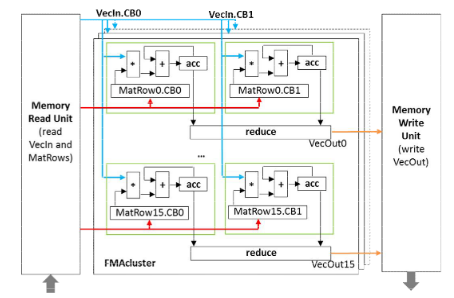
\includegraphics[width=\linewidth]{pictures/fpga_operations.png}
		\label{fig:fpgahw}
	\end{figure}
	\\
	Microsoft found a use case for FPGAs in their datacenter for the inference phase in their Azure Cloud. The Bing ranking was accelerated by a factor of nearly 2 by using FPGAs instead of traditional hardware \cite{putnam2014reconfigurable}. Further work was done to achieve even better performance \cite{ovtcharov2015accelerating}. A key feature of the updated hardware is the ability to support many different configurations of the hardware without having to recompile, allowing for a faster design process. The circuit is composed of many different processing elements as well as buffers. The processing elements can be scaled up to a margin of more units, through their partly independent structure, to achieve faster processing times. Input data is moved from the DRAM into an input buffer. A software unit distributes the data across the processing elements, which perform independent operations. The results are stored in the weight buffer.
	\\
	The buffers allow together with the network-on-chip to distribute data across the unit. This reduces the network traffic to and from outside of the chip, by making use of the buffers. 
	\\
	
	\section{Application-Specific Integrated Circuit}
	\begin{table*}[!b]
		\renewcommand{\arraystretch}{1.3}
		\centering
		\caption{A Table showing some results from the training in MLPerf v0.7 in the category Regular, Closed Division Times \cite{mlperfresults}. While this data is very simplified Real caption\textsuperscript{*}, the full data can be viewed on the official Website.}
		\begin{tabular}{lllllll}
			\toprule
			\bfseries HW Accelerator                            & \bfseries Amount & \bfseries \thead[l]{Image \\ Classification}       & \bfseries \thead[l]{Object detection \\ light-weight}    & \bfseries \thead[l]{Translation \\ recurrent}    & \bfseries \thead[l]{Natural Language \\ Processing}     & \bfseries \thead[l]{Reinforcement \\ Learning}      \\
			\midrule
			Google TPUv3 (in Cloud)                   & 16     & 28.71   &      &      & 56.74 &        \\
			Google TPUv3                              & 512    &         &      & 2.1  &       &        \\
			Google TPUv3                              & 4096   & 0.48    & 0.46 &      & 0.39  &        \\
			Google TPUv4                              & 256    & 4.5     & 1.43 & 2.08 & 5.73  & 150.95 \\
			NVIDIA   A100-SXM4-40GB (400W)            & 1840   & 0.76    &      &      &       &        \\
			NVIDIA   A100-SXM4-40GB (400W)            & 1024   &         & 0.82 & 0.71 &       &        \\
			NVIDIA   A100-SXM4-40GB (400W)            & 2048   &         &      &      & 0.81  &        \\
			NVIDIA   A100-SXM4-40GB (400W)            & 1792   &         &      &      &       & 17.07  \\
			Huawei Ascend910                          & 512    & 1.56    &      &      &       &        \\
			Intel   Xeon Platinum 8380H CPU @ 2.90GHz & 8      & 1104.53 &      &      &       &		\\
			\bottomrule                              
		\end{tabular}
		\rule{0pt}{3ex} 
		\small\textsuperscript{*} The different results include different configurations for each hardware accelerator
		\label{table:mlperf}
	\end{table*}
	
	Although an Application-Specific Integrated Circuit (ASIC) shares similarities with a FPGA, they are fundamentally different \cite{capra2020updated}. The most notable difference is that while FPGAs can be reprogrammed after production, this is not the case for ASICs, rather are they designed for a specific cause that will remain the same over their lifetime. To add on their design process is also more complicated and requires more time. Their edge compared to FPGAs is better optimization and energy efficiency, perfecting the hardware-specific advantages of FPGAs.
	\\
	Google started working on an own custom ASIC, after observing that only a three minutes of speech search (using neural networks) would double their computational capacity \cite{jouppi2017datacenter}. Making this the use-case the hardware was therefore built specifically for the inference phase. The work became the Tensor Processing Unit (TPU) released in 2016. The main components of the first version included a Matrix Multiply Unit (MMU), a Unified Buffer and Accumulators. The Matrix Multiply Unit contains 256x256 multiplier-accumulators (MACs), which perform 8-bit operations, whose results are stored in accumulators. Many scientific works have shown that during the inference phase lower numerical precision (lower than the usual 32-bit floating point) can be used to achieve faster training times without loss of accuracy\cite{rodriguez2018lower}. This makes the Matrix Multiply Unit a good tool to process the data coming through the layers. Since the TPU is only used for inference Google implemented a Weight FIFO, which is read-only and makes accessing the weights needed in the MMU fast. The transitional results are at the end stored in the Unified Buffer. For faster processing a systolic array was used, which reduces read and write operations. 
	Another way the hardware accelerates is by using a 4-stage pipeline parallelism.
	\begin{figure}[h]
		\caption{A simplified block diagram of the first version TPU. The left side represents the host (CPU). The host sends instructions to the TPU and receives a data back \cite{jouppi2017datacenter}.}
		\centering
		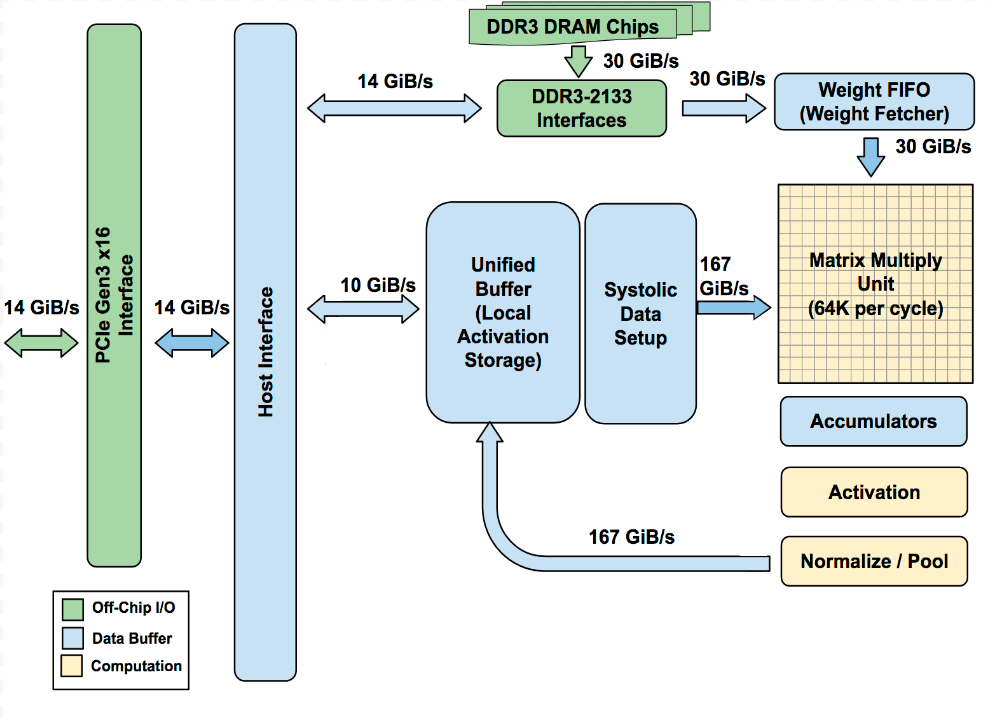
\includegraphics[width=\linewidth]{pictures/tpu_floorplan.png}
	\end{figure}
	\\
	Since the release of the first version Google released two newer versions and also announced the work on a fourth version:
	\begin{itemize}
		\item The TPUv2 was built from the ground up working on problems of the first version. The release of the second version focused mostly on higher memory bandwidth and even faster processing, containing two Matrix Execution Units \cite{secondversiontpu}. The second version was now also able to support training models. Another addition was the so-called TPU Pods, which are essentially multiple TPU devices connected together. In a TPU Pod the units are connected in such a way that the workload between the different devices can be split up autonomously, meaning without the help of a host CPU.
		\item The TPUv3 improved similar aspects as its predecessor, having four Matrix Execution Units \cite{thirdversiontpu}.
		\item  Google has announced that it is working on bringing out a fourth version of their TPU, claiming to be 2.7x faster than their third version \cite{fourthversiontpu}.
	\end{itemize}
	
	
	\section{Comparison Accelerators}
	The comparison between ASICs, FPGAs and GPUs will be divided into two main aspects: firstly a general comparison between the different accelerators regarding often used measures and secondly an insight into the research regarding hardware accelerators for neural networks. The comparison will focus predominantly on the hardware used in datacenters.
	\\
	The main metrics for measuring hardware accelerators are performance, energy efficiency and memory bandwidth.
	\\
	
	\textbf{Performance}:
	The performance (often also called the throughput) determines how often the hardware performs a complete convolution/a complete inference is performed on the hardware. Most of the times this metric is measured in billions of operations per second (GOP/s). Other alternatives include billions of Macs per second (GMAC/s) or the amount of inferences achieved (e.g. when talking about image classification the hardware classified x images/second). 
	\textbf{Energy Efficiency}:
	The energy efficiency is the power the unit bestows put in ration with the performance. This is an important unit for edge devices, as power is often a limited source for these devices.
	
	\textbf{Memory Bandwidth} is simply the rate at which the hardware can read/write data.
	The accuracy is also a metric cited, but it will not be discussed since the software is the contributing factor for this.
	\\
	\\
	Measuring these standard metrics on different hardware accelerators can be challenging \cite{capra2020updated}. Most of the scientific work is only presented on the target application, making good benchmarking between different accelerators hard. Results of benchmarks with different neural networks or different data cannot be reasonably compared.
	There are different scientific works that are dedicated to creating frameworks for benchmarking hardware accelerators \cite{chen2012benchnn} \cite{zhu2018benchmarking} \cite{blott2019qutibench} \cite{dong2017dnnmark}. The most accredited is MLPerf, which claims to be the industry standard for measuring the performance of hardware accelerators for neural networks\cite{mattson2020mlperf}. It was founded in 2018 and is being worked on by both, members of science and industry, including Google, NVIDIA, Harvard University and Stanford University to name a few. The specific implementation of the MLPerf Framework would overreach the premise of this paper, as such I will focus on the results.
	A peak into the results can be seen in Table \ref{table:mlperf}. NVIDIA had 85\% of the submission, which include many different variants of their A100 GPU and others \cite{mlperfresultshpc}. The NVIDIA A100 performs the best for both training and inference phase Per-Accelerator. Google has the Max Scale Record with 4096 units of their TPUv3. In comparison, the Intel Processor is in the 100x slower than the GPU \cite{mlperfresultsnvidia}. 
	\\
	GPUs are widely used being called the "workhorses" for Machine Learning\cite{capra2020updated}, being among the most used for Machine Learning \cite{mostusedgpu}. There are a lot of frameworks for working with GPUs on Machine Learning, they are very accessible and perform well. To add on they are mostly implemented on the software level, which as referenced in \autoref{section:foo} is easier to work on, when having a software background.  Since most of the applications such as speech and image computation is being done in the cloud \cite{sze2017efficient} the hardware in big tech companies is being used for the direct application of neural networks.
	\\
	A metric that is not represented in the MLPerf benchmark is the energy efficiency. Here FPGAs seem to have an advantage thanks to their efficient pathing of data and operating. In scientific research, as well as the benchmark QuTiBench\cite{blott2019qutibench} referenced earlier, FPGAs have a better performance/power than the other methods, in some cases up to 10x better than GPUs \cite{ovtcharov2015accelerating} \cite{capra2020updated}. 
	\\
	\\
	The second aspect to consider is the scientific research. A detailed systematic literature review examined scientific papers between the years 2009 and 2019 \cite{talib2020systematic}. The most commonly used accelerator was FPGA, followed by the GPU \ref{fig:piech}. The study concluded that the reason was the fast prototyping, as well as the recent rise in accessibility that made FPGAs popular for researchers. ASICs on the other hand, are higher prized compared to GPUs and FPGAs.
	
	\begin{figure}
		\caption{The results percentages of the different hardware accelerators found in scientific papers \cite{talib2020systematic}. Compare in the pie chart refers to comparison studies.}
		\label{fig:piech}
		\centering
		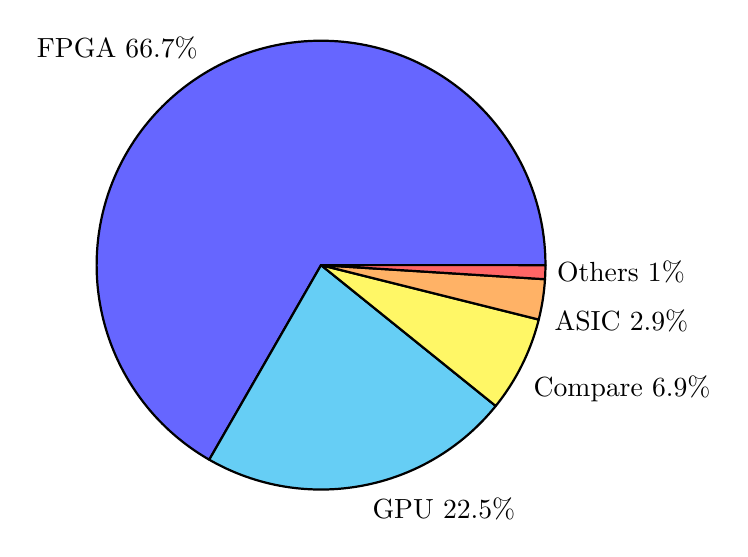
\begin{tikzpicture}[scale=0.95]
			\pie[hide number]{66.7/FPGA 66.7\%, 22.5/GPU 22.5\%, 6.9/Compare 6.9\%, 2.9/ASIC 2.9\%, 1/Others 1\%}
		\end{tikzpicture}
	\end{figure}
	
	\section{Hardware Accelerators in Edge Devices}
	Although it is not directly a specific type of hardware, hardware accelerators in edge devices play a key role in bringing the services of neural networks to the application. The application for neural networks is, as mentioned in the introduction, manifold. Many applications need fast response times (e.g. autonomous driving) and cannot rely on cloud computing solutions alone. This results in the need for the computation to happen right at the source resulting in the need for hardware accelerators in edge devices. This does not mean that cloud is not used at all, rather the edge device works together with the cloud.
	\\
	The hardware accelerators built into edge devices have different demands than those in datacenters \cite{wang2020convergence}. The units in edge devices face limits on the computation available and the energy consumption. The devices are also far smaller. This leads to a lot of tradeoffs between the different architectures often small microcontrollers. FPGAs have lower power consumption, can be better optimized for specific applications and have better timings \cite{jiang2018accelerating}. GPUs/CPUs have more stable architecture and better floating point capabilities \cite{chen2019exploring}. Some concrete examples include a Neural Processing Unit from Siemens, that enables Artificial Intelligence for automation task in manufacturing \cite{siemensnpu} or a special 8-core neural engine in the iPhone dedicated for image processing \cite{applenpu}.
	\\
	
	\section{Conclusion}
	The hardware in neural networks plays a key role in bringing neural networks to the broad spectrum of its usage, as well as help in making better and smarter neural networks. In this paper the tradeoffs for each of the different methods can be seen. Each of the hardware accelerators have different advantages and disadvantages that make them suitable in their usable environment, which is why choosing the right hardware should be a crucial decision when using neural networks. The different methods for accelerating neural networks have been and are still being optimized to achieve good performance. With the rise of the Internet of Things, more energy-efficient devices will be needed to precisely meet the demands for these devices. The challenge here will be to juggle networking, processing power, and energy consumption with the best performance of the neural network.
	\newpage
	\bibliography{References}
\end{document}
